\documentclass{article}
\usepackage{amsmath}
\usepackage{graphicx}
\usepackage{siunitx}
\usepackage{physics}
\usepackage{graphicx}
\usepackage{float}
\sisetup{output-exponent-marker=\ensuremath{\mathrm{e}}}

\title{Balanza de Corriente}
\author{Estudiante de Física}
\date{\today}

\begin{document}

\maketitle

\section{Objetivo}
\begin{itemize}
    \item Estudiar la \textbf{ley de Laplace} aplicada a la interacción entre corrientes eléctricas y campos magnéticos.
    \item Determinar experimentalmente el \textbf{módulo del campo magnético} generado por un imán permanente.
    \item Observar y analizar el \textbf{principio de acción y reacción} de Newton en un sistema magnético.
\end{itemize}

\section{Materiales}
\begin{itemize}
    \item \textbf{Generador de corriente continua}: Para suministrar una corriente estable.
    \item \textbf{Balanza digital}: Medir variaciones de masa debido a fuerzas magnéticas.
    \item \textbf{Soporte y barra metálica}: Estructura para fijar componentes.
    \item \textbf{Set de circuitos impresos} (6 modelos): Diferentes longitudes de conductores para variar el parámetro \( L \).
    \item \textbf{Unidad de sujeción}: Dispositivo para fijar los circuitos impresos cerca del imán.
    \item \textbf{Cables y amperímetro}: Conectar y medir la corriente en el circuito.
    \item \textbf{Imán permanente}: Fuente del campo magnético.
\end{itemize}

\section{Fundamentos Teóricos}
\subsection{Ley de Laplace}
Cuando un conductor de longitud \( L \), por el que circula una corriente \( I \), se coloca en un campo magnético \( \vec{B} \), experimenta una fuerza magnética \( \vec{F} \). Esta fuerza es perpendicular al plano formado por \( \vec{B} \) y el vector longitud \( \vec{L} \), y se expresa como:

\[
\vec{F} = I \cdot (\vec{L} \times \vec{B}) \quad \text{(1)}
\]

Donde:
\begin{itemize}
    \item \( \vec{L} \): Vector con magnitud igual a la longitud del conductor y dirección igual al sentido de la corriente.
    \item \( \vec{B} \): Campo magnético del imán.
\end{itemize}

\section{Procedimiento Experimental}
\subsection{Montaje Inicial}
\begin{enumerate}
    \item \textbf{Fijación de componentes}:
    \begin{itemize}
        \item Unir la barra metálica a la base del soporte.
        \item Enroscar la unidad de sujeción en la barra.
        \item Acoplar el circuito impreso seleccionado en la parte frontal de la unidad de sujeción.
    \end{itemize}
    
    \item \textbf{Configuración eléctrica}:
    \begin{itemize}
        \item Conectar el generador en \textbf{modo corriente continua}.
        \item Colocar el amperímetro en serie entre el generador y la unidad de sujeción.
        \item Asegurar que el circuito esté abierto hasta comenzar las mediciones.
    \end{itemize}
\end{enumerate}

\subsection{Medición de la Masa del Imán}
\begin{itemize}
    \item Pesar el imán con la balanza y registrar su masa (\( m \)) junto con la precisión del instrumento.
\end{itemize}

\subsection{Colocación del Circuito Impreso}
\begin{itemize}
    \item Posicionar el circuito impreso entre los polos del imán \textbf{sin contacto físico} (Figura 
    \item Asegurar que solo la sección horizontal del circuito esté expuesta al campo magnético.
\end{itemize}

\subsection{Ejecución del Experimento}
\begin{enumerate}
    \item Encender el generador para establecer una corriente \( I \) en el circuito.
    \item Registrar la \textbf{masa aparente} (\( m' \)) mostrada por la balanza, que disminuirá debido a la fuerza de reacción magnética \( \vec{F}_r \).
\end{enumerate}

\subsection{Análisis de Fuerzas}
En equilibrio estático, las fuerzas sobre el imán cumplen:

\[
\sum \vec{F}_i = \vec{F}_N + \vec{P} + \vec{F}_r = \vec{0} \quad \text{(2)}
\]

Donde:
\begin{itemize}
    \item \( \vec{F}_N \): Fuerza normal de la balanza.
    \item \( \vec{P} = m \cdot \vec{g} \): Peso del imán.
    \item \( \vec{F}_r = I \cdot L \cdot |\vec{B}| \): Fuerza de reacción (módulo igual a la fuerza magnética).
\end{itemize}

La relación entre la masa aparente y el campo magnético se obtiene de:

\[
m' \cdot g = m \cdot g - I \cdot L \cdot |\vec{B}| \quad \text{(6)}
\]

\section{Tratamiento de datos}
\subsection{Intensidad constante}
Teniendo en cuenta la anterior dependencia

\[
    F_N = m'g
\]
podemos desarrollar la propagación de errores
\[
    \Delta F_N = |\pdv{F_N}{m'}|\Delta m' +|\pdv{F_N}{g}|\Delta g = g\Delta m' + m'\Delta g
\]
sabiendo que \(\Delta g =10^{-7}\) y que \(\Delta m' = 10^-6\), este error acaba siendo apróximadamente \(\Delta F_N = 10^-4~(N)\).
Además, la longitud de los circuitos $L$ se midió con un pie de rey que tenía una precisión de $\Delta L =10^{-5}$.
Con esto tenemos los siguientes datos:
\begin{table}[H]
    \begin{tabular}{l|l|l|l|l}
    $I~(A)$ & $m~(kg)$                       & $F_N~(N)$         & $L~(m)$             & Circuito \\
    \hline
    $1.5\pm0.01$     & $(160.27\pm 0.01)\num{e-3}$ & $1.5706\pm0.0001$ & $(7.80\pm 0.01)\num{e-3}$ & SF40\\
    \hline
    $1.5\pm0.01$ & $(160.11\pm 0.01)\num{e-3}$ & $1.5690\pm 0.0001$ & $(20.10\pm 0.01)\num{e-3}$ & SF37\\
    \hline
    $1.5\pm0.01$ & $(160.03\pm 0.01)\num{e-3}$ & $1.5682\pm 0.0001$ & $(27.52\pm0.01)\num{e-3}$ & SF39\\
    \hline
    $1.5\pm0.01$ & $(159.76\pm 0.01)\num{e-3}$ &  $1.5655\pm 0.0001$ & $(30.00\pm0.01)\num{e-3}$ & SF38\\
    \hline
    $1.5\pm0.01$ & $(159.65\pm0.01)\num{e-3}$ & $1.5645\pm0.0001$ & $(37.75\pm0.01)\num{e-3}$ & SF41\\
    \hline
    $1.5\pm0.01$ & $(159.13\pm0.01)\num{e-3}$ & $1.5594\pm0.0001$ & $(40.00\pm0.01)\num{e-3}$ & SF42
    \end{tabular}
    \end{table}
Si representamos $F_N$ frente a $L$, obtenemos
\begin{figure}[H]
    \centering
    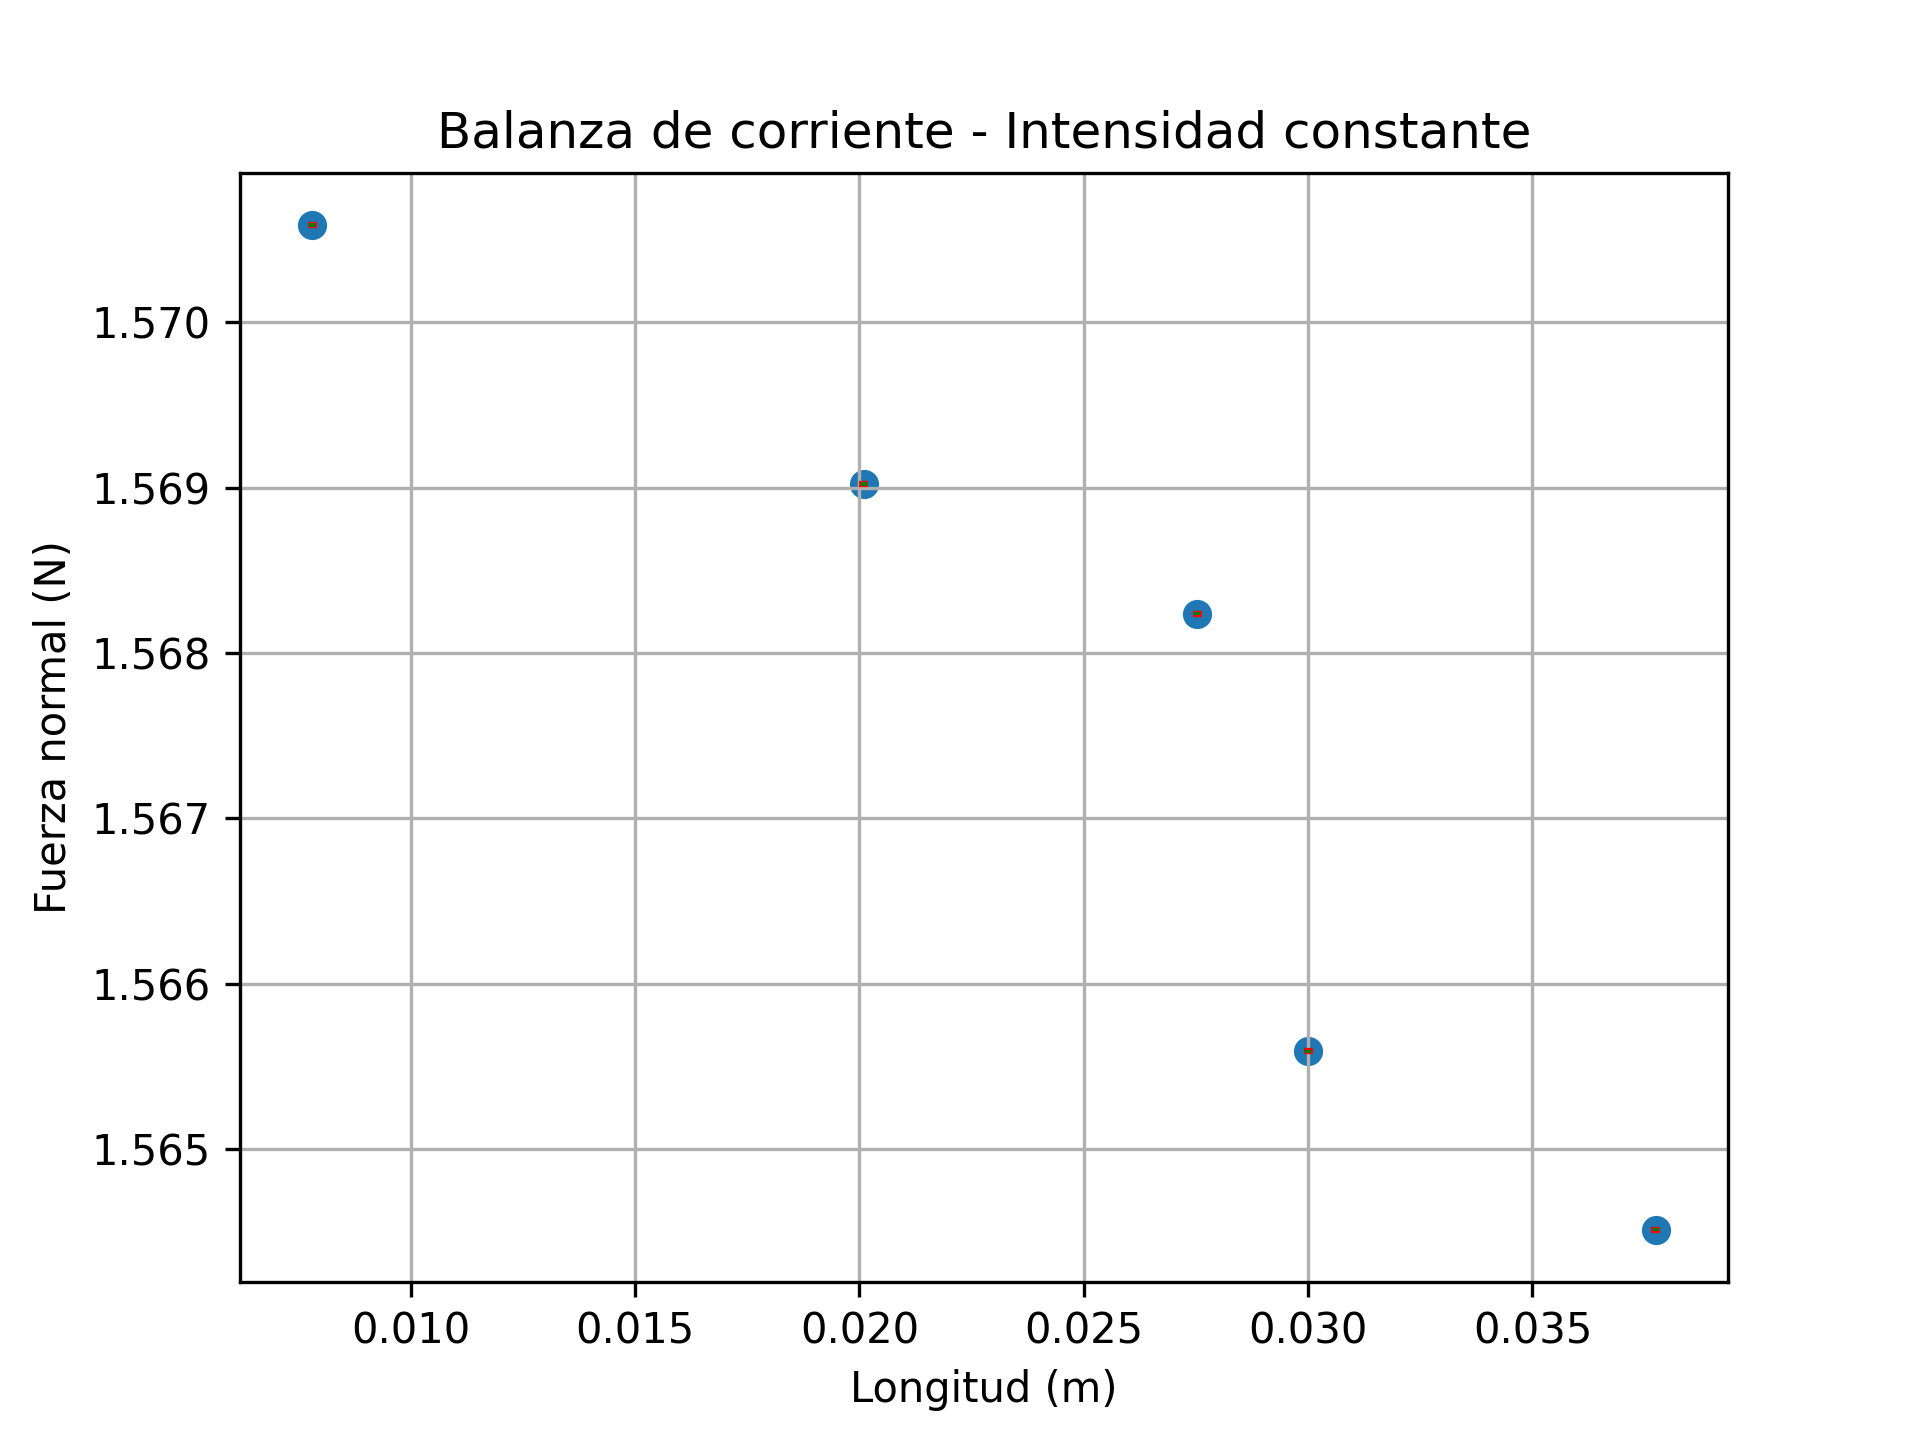
\includegraphics[scale=0.75]{images/f_n_contra_l.png}
\end{figure}
Donde se puede observar una clara dependencia lineal. Para el ajuste lineal, vamos a obtener una recta de la forma
\[
    F_N = n + L\cdot m
\]
donde $n$ va a tener unidades de fuerza, y $m$ va a tener unidades de fuerza por unidad de longitud. Concretamente,
esta $m$ será
\[
    m = IB
\]
Realizando este ajuste, obtenemos que $n = 1.572\pm 0.001~(N)$ y que $m = -0.21\pm 0.04~(\frac{N}{m})$, 
además de un coeficiente de correlación $r =-0.9390$.\\
Para deducir el valor del campo magnético en base a la pendiente, obtenemos que:
\[
    B = \frac{m}{I} = -0.14~(T)
\]
Desarrollamos la propagación de errores:
\[
    \Delta B = |\pdv{B}{m}|\Delta m + |\pdv{B}{I}|\Delta I = \frac{\Delta m}{I}+ \frac{m}{I^2}\Delta I\approx 0.03
\]
Finalmente, nuestro campo magnético es
\[
    \boxed{
        B = -0.14\pm0.03~(T)
    }
\]
Respecto a la masa del imán, sabemos que la ordenada en el origen $n$ es
\[
    n = mg
\]
por lo que podemos despejar para obtener
\[
    m = \frac{n}{g}
\]
Desarrollando la propagación del error, obtenemos que
\[
    \Delta m = |\pdv{m}{n}|\Delta n +|\pdv{m}{g}|\Delta g = \frac{\Delta n}{g} + \frac{n}{g^2}\Delta g = \frac{0.001}{9.7996413} + 
    \frac{1.572}{9.7996413^2}\cdot 0.0000001 \approx 0.0001
\]
Por lo que la masa del imán es
\[
    m = 0.1604\pm0.0001
\]
Si calculamos el error porcentual en comparación con la masa medida en el laboratorio $(m = 0.16041)$, nuestro error es
\[
    \varepsilon_P = |\frac{m-\tilde{m}}{m}|\cdot 100 \approx 0.006\%
\]
\subsection{Circuito constante}
Cuando se fue variando la intensidad y se mantuvo el circuito constante, se obtuvieron los siguientes datos:
\begin{table}[H]
    \begin{tabular}{l|l|l|l|l}
        $I~(A)$ & $m~(kg)$ & $F_N~(N)$ & $L~(m)$ & Circuito\\
        \hline
        $1.75\pm0.01$ & $(159.64\pm0.01)\num{e-3}$ & $1.5644\pm0.0001$&$(30.00\pm0.01)\num{e-3}$&SF38\\
        \hline
        $2\pm0.01$&$(159.56\pm0.01)\num{e-3}$&$1.5636\pm0.0001$&$(30.00\pm0.01)\num{e-3}$&SF38\\
        \hline
        $2.25\pm0.01$&$(159.47\pm0.01)\num{e-3}$&$1.5627\pm0.0001$&$(30.00\pm0.01)\num{e-3}$&SF38\\
        \hline
        $2.5\pm0.01$&$(159.36\pm0.01)\num{e-3}$&$1.5616\pm0.0001$&$(30.00\pm0.01)\num{e-3}$&SF38\\
        \hline
        $2.75\pm0.01$&$(159.26\pm0.01)\num{e-3}$&$1.5606\pm0.0001$&$(30.00\pm0.01)\num{e-3}$&SF38\\
        \hline
        $3.00\pm0.01$&$(159.14\pm0.01)\num{e-3}$&$1.5595\pm0.0001$&$(30.00\pm0.01)\num{e-3}$&SF38
    \end{tabular}
\end{table}
Lo que nos da la siguiente gráfica:
\begin{figure}[H]
    \centering
    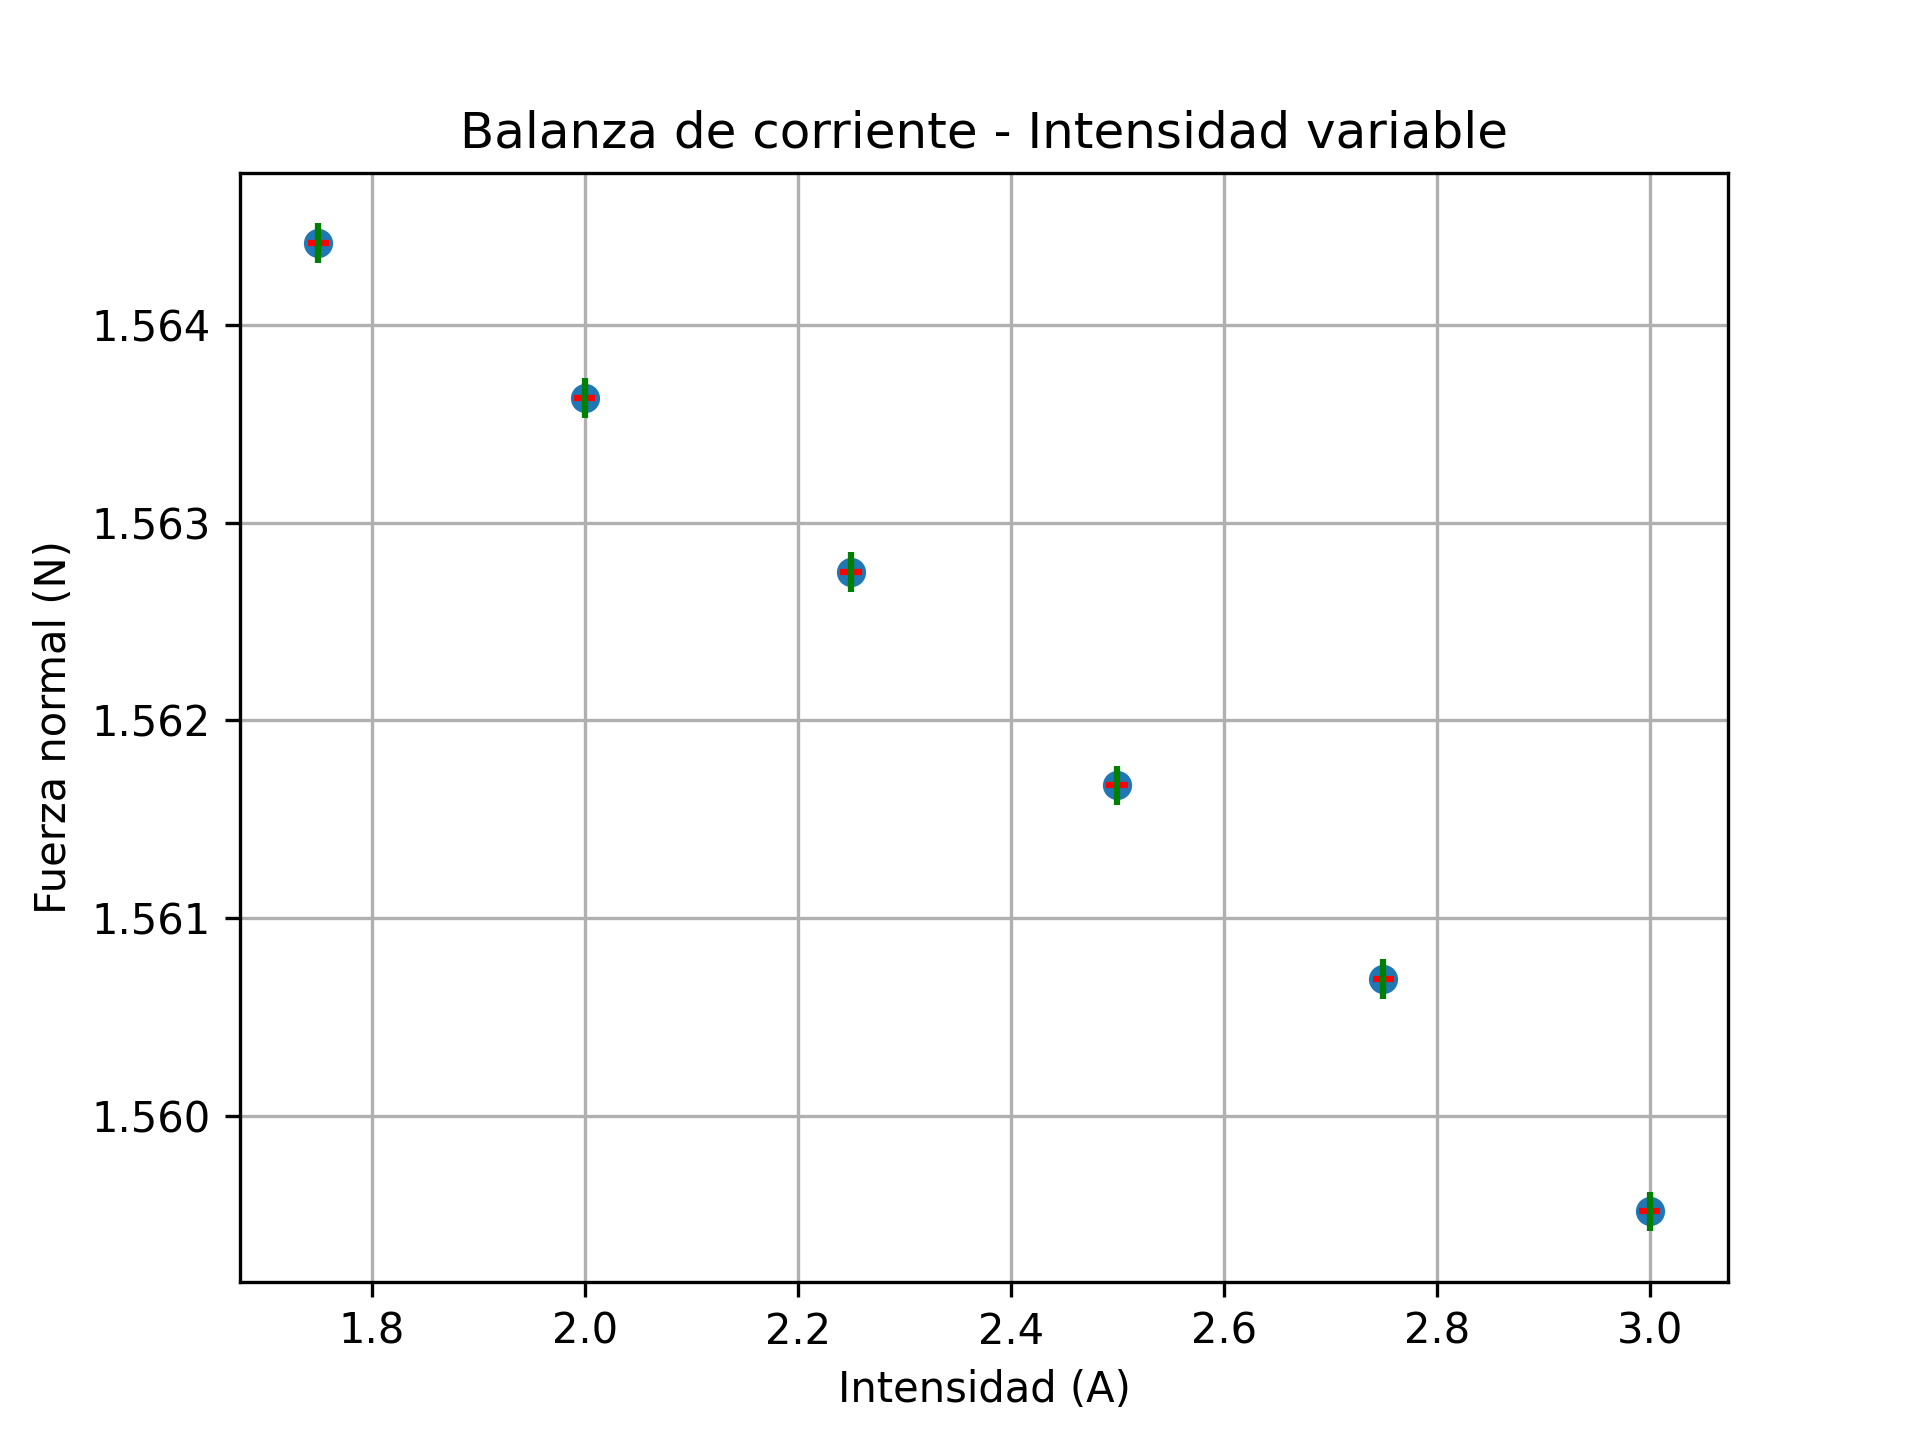
\includegraphics[scale=0.75]{images/f_n_contra_i.png}
\end{figure}
Donde la dependencia lineal es todavía más evidente. Realizando el ajuste de mínimos cuadrados, obtenemos una ordenada en el origen
$n =1.5714\pm 0.0003~(N)$, y una pendiente $m=-0.0039\pm0.0001~(\frac{N}{A})$, además de un coeficiente de correlación $r =-0.9979$. De nuevo,
tenemos una recta de la forma
\[
    F_N = n + I\cdot m
\]
donde en este caso $m = BL$. Podemos despejar $B$ para obtener
\[
    B = \frac{m}{L} = -0.13~(T)
\]
Desarrollando la propagación de errores, obtenemos
\[
    \Delta B = |\pdv{B}{m}|\Delta m + |\pdv{B}{L}|\Delta L = \frac{\Delta m }{L} + \frac{m}{L^2}\Delta L = 
    \frac{0.0001}{0.03}+\frac{0.0039}{0.03^2}\cdot 10^{-5}\approx 0.003~(T)
\]
por tanto, nuestro campo magnético es
\[
    B = -0.13\pm 0.003~(T)
\]
Para calcular la masa del imán, tenemos que $n = m'g$, por lo que podemos despejar para obtener
\[
    m' = \frac{n}{g}=0.16035
\]
Calculamos el error:
\[
    \Delta m' = |\pdv{m'}{n}|\Delta n +|\pdv{m'}{g}|\Delta g = \frac{\Delta n}{g} + \frac{n}{g^2}\Delta g = \frac{0.0003}{9.7996413} + 
    \frac{1.5714}{9.7996413^2}\cdot 0.0000001 \approx 0.00003
\]
Por tanto, la masa es
\[
    m' = 0.16035\pm0.00003
\]
Comparado con el resultado observado en el laboratorio, nuestro error porcentual es
\[
    \varepsilon_P = |\frac{m-\tilde{m}}{m}|\cdot 100 \approx 0.04\%
\]
\end{document}